% textidote: ignore begin
\subsection{Class Diagrams}\label{subsec:class-diagrams}
% textidote: ignore end

The following section will describe the most important models in the system.
This is done to give a better understanding of the architecture, more specifically the business logic.

% textidote: ignore begin
\subsubsection{Components}
% textidote: ignore end

As seen in Figure~\ref{fig:model-class-diagram}, the model describes the repository layer.
This layer connects both to the csv handler, but also the database as it uses the models to persist data.

\begin{figure}[H]
    \centering
    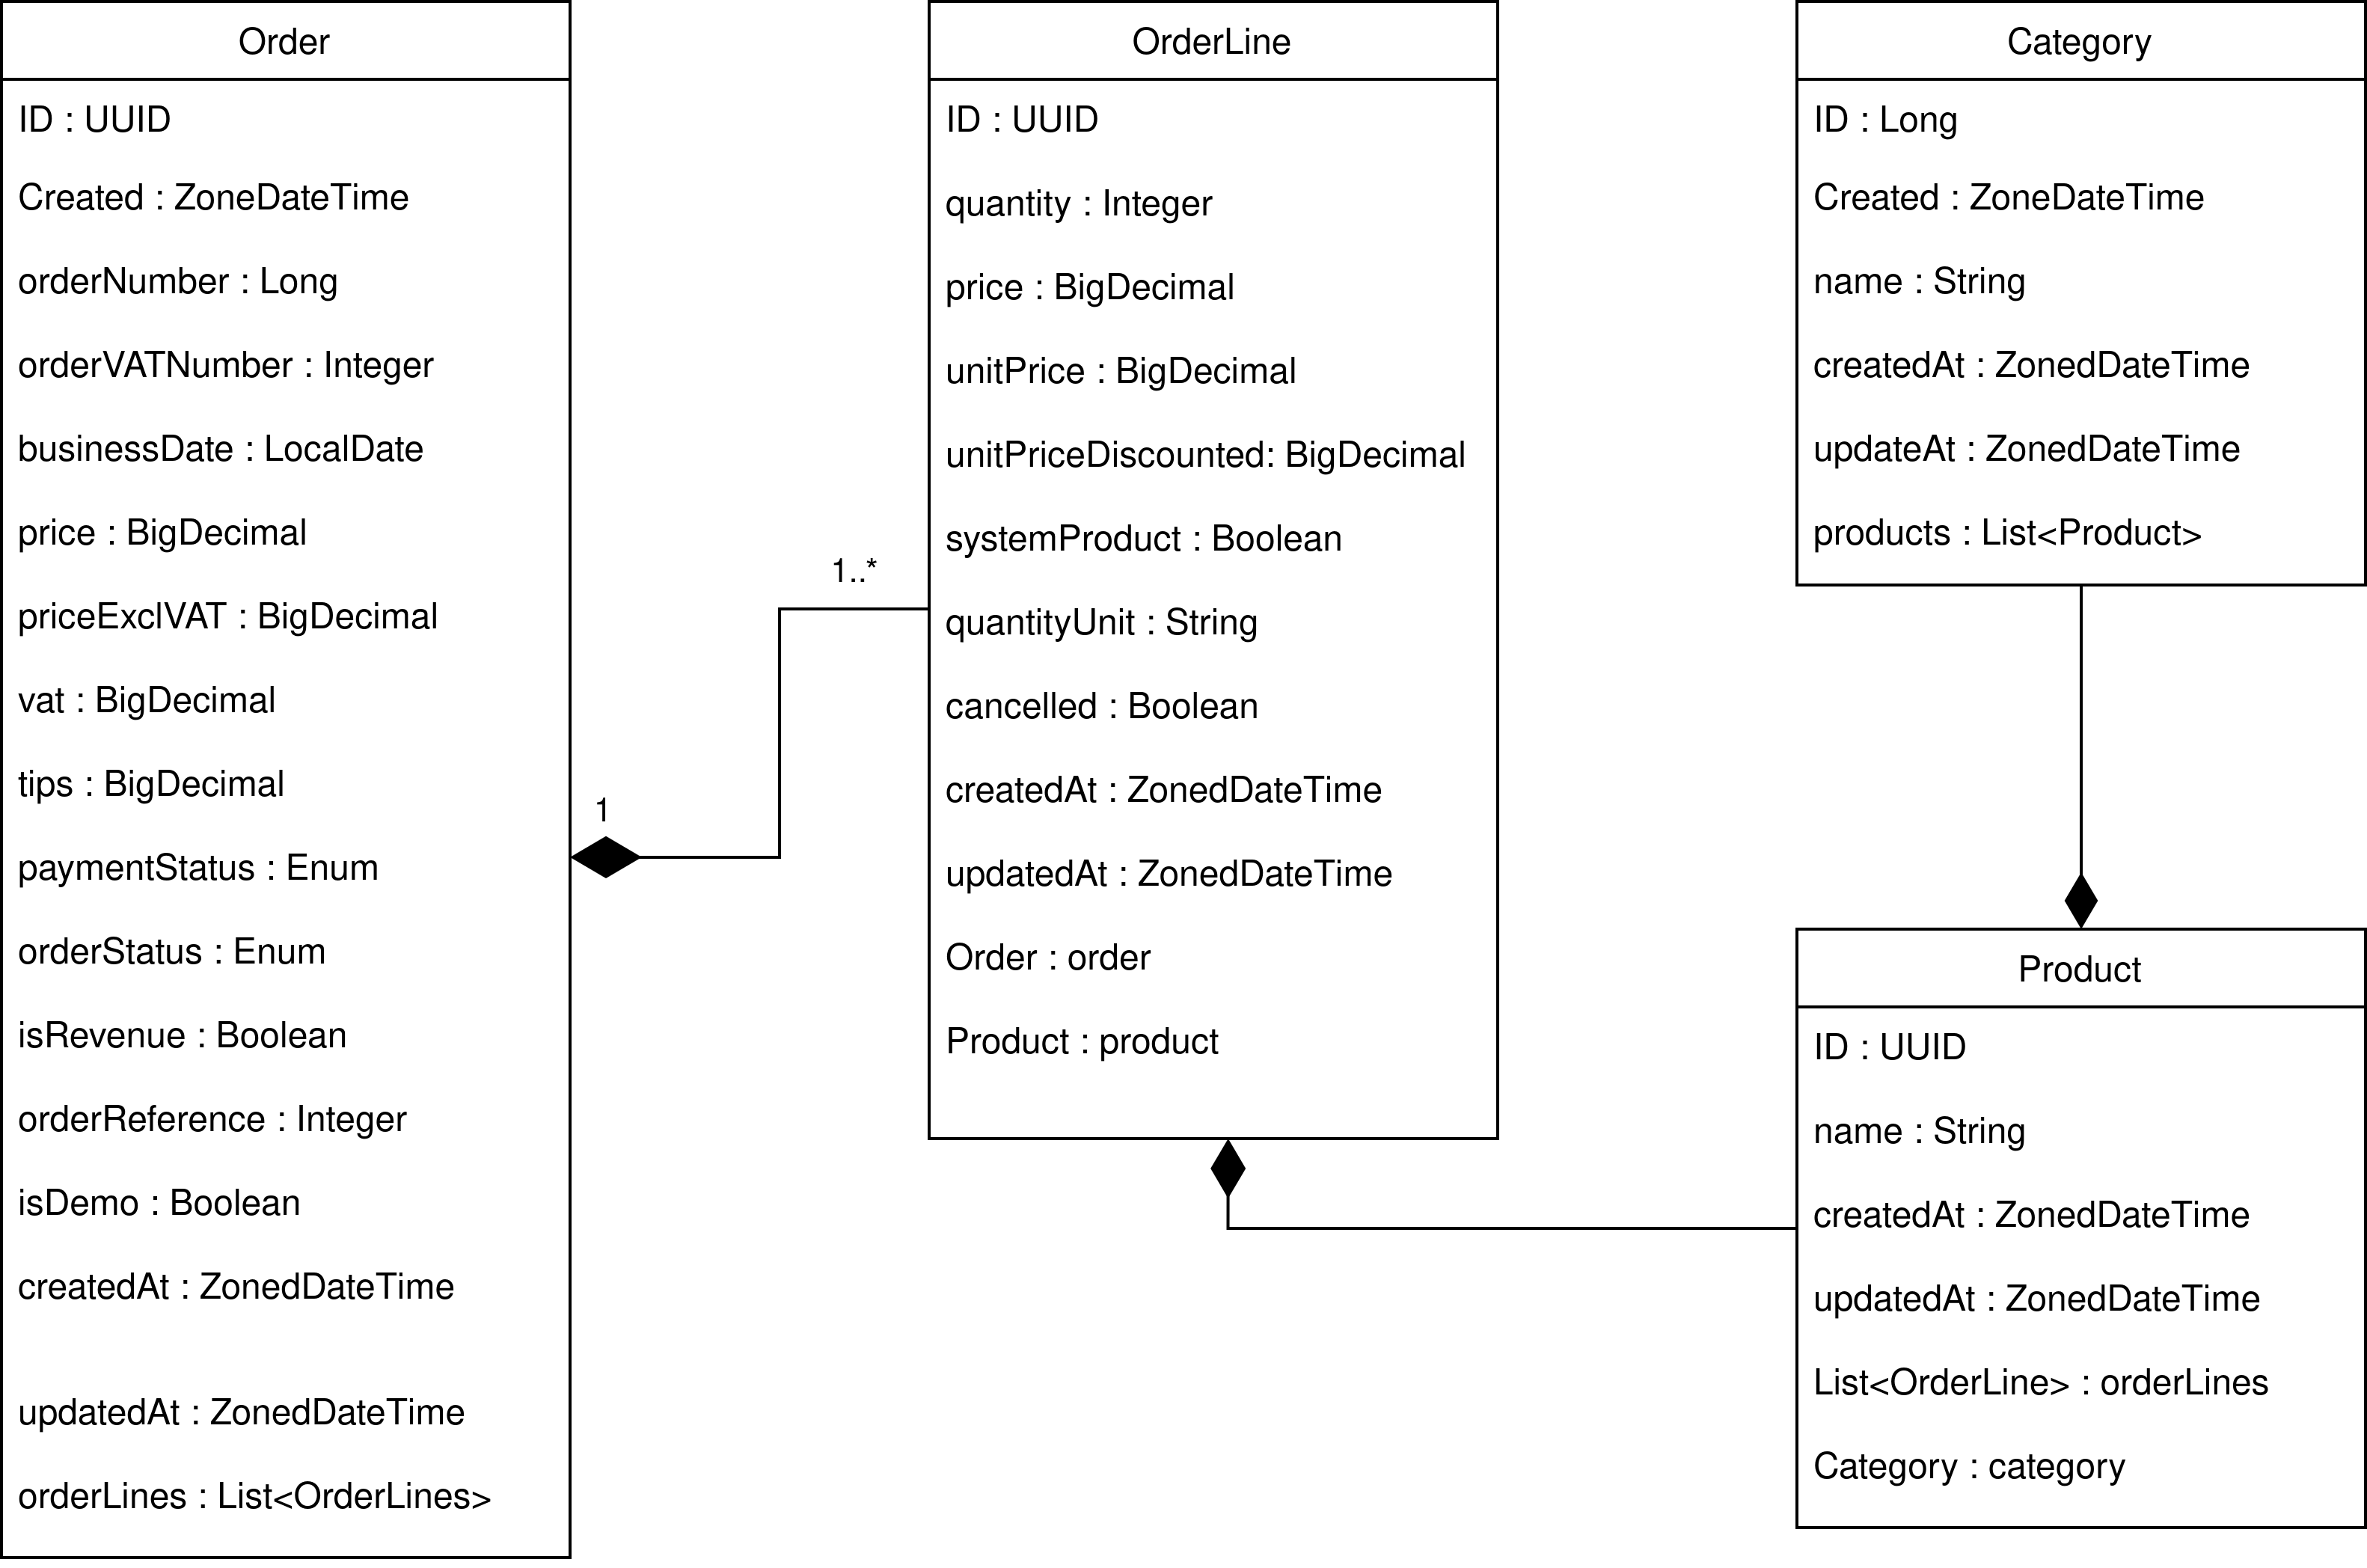
\includegraphics[width=\textwidth]{model-class-diagram}
    \caption{Class diagram of the model, getter and setter methods are excluded.
    }\label{fig:model-class-diagram}
\end{figure}

% textidote: ignore begin
\subsubsection{Architecture}
% textidote: ignore end

As seen in Figure~\ref{fig:architechture-class-diagram}, the model describes the component architecture and component
design.
This is a further abstraction from Figure~\ref{fig:model-class-diagram}, where also the interfaces and other components
are displayed.

\begin{figure}[H]
    \centering
    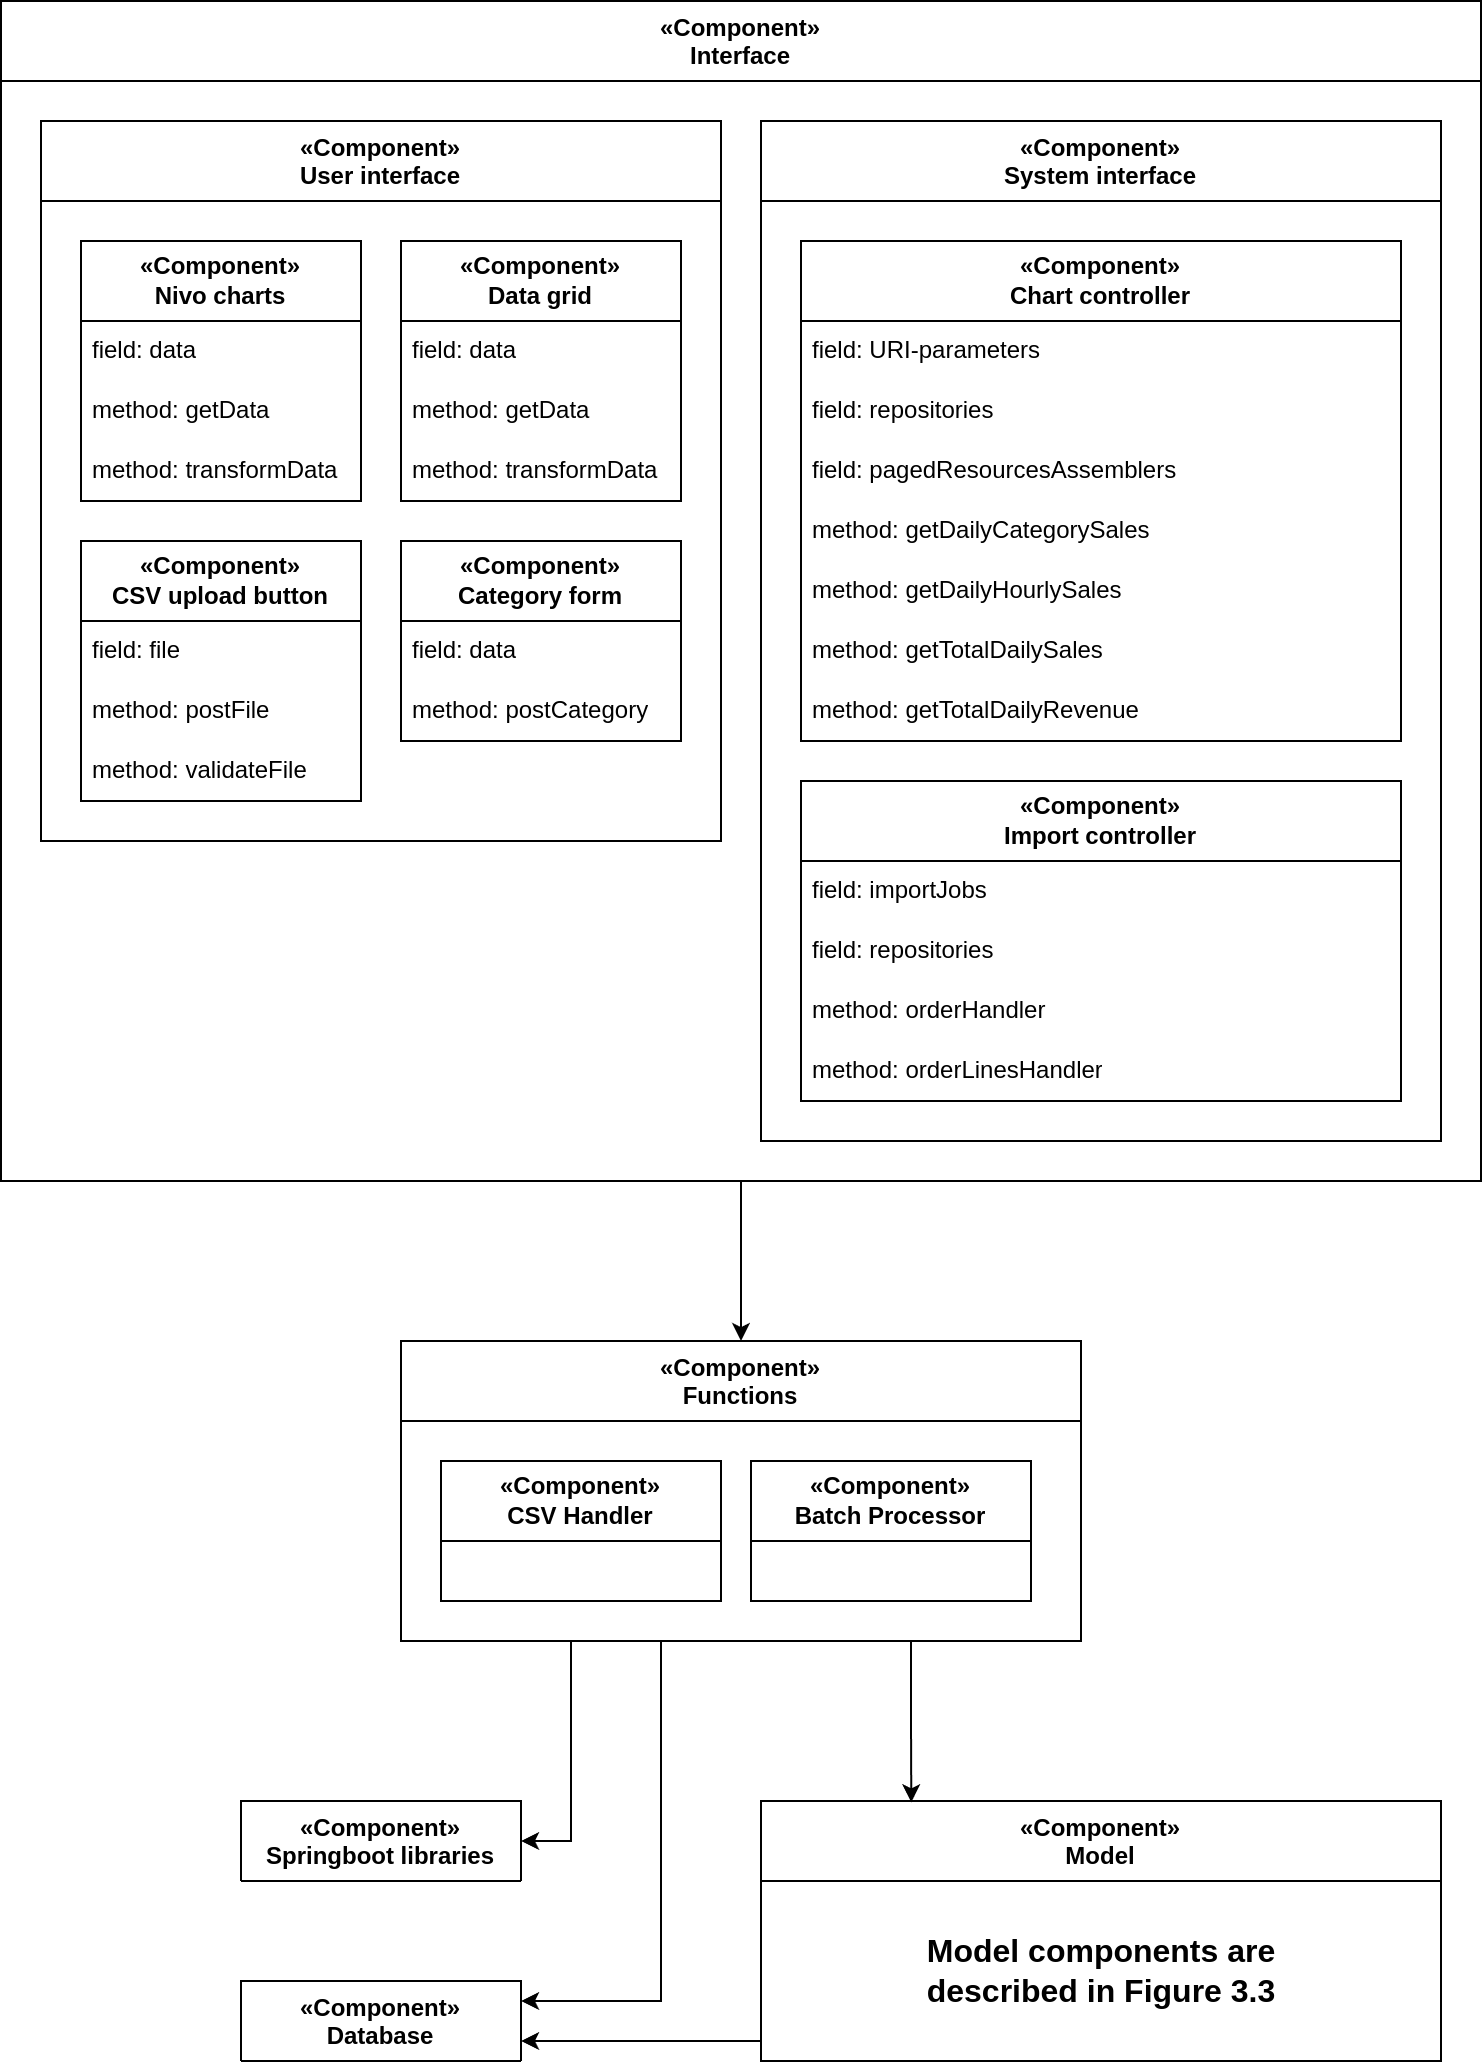
\includegraphics[width=\textwidth]{architecture-class-diagram}
    \caption{Class diagram of the architechture.
    }\label{fig:architechture-class-diagram}
\end{figure}
